\subsection{Leibniz’s Differentials: Infinitesimals and Ratios}  

While Newton thought of calculus in terms of motion and geometry, Leibniz approached it algebraically. He treated differentiation as a symbolic ratio of infinitesimally small changes — not tied to physical motion, but to abstract relationships between variables. His notation, elegant and general, became the standard language of calculus:

\[
dy = \frac{dy}{dx} dx
\]

where:  
\begin{itemize}
    \item \( dx \) is an infinitesimal change in \( x \).  
    \item \( dy \) is an infinitesimal change in \( y \).  
    \item \( \frac{dy}{dx} \) is the derivative, which represents the curve’s local slope.  
\end{itemize}  

\begin{figure}[H]
\centering
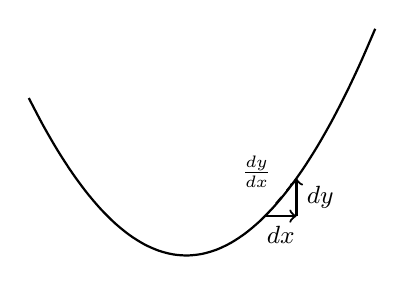
\begin{tikzpicture}[scale=2]
    % Draw curve
    \draw[thick, domain=-1:1.2, smooth, variable=\x] plot ({\x},{\x*\x});

    % Draw differentials
    \draw[->, thick] (0.5, 0.25) -- (0.7, 0.25) node[midway, below] {\small $dx$};
    \draw[->, thick] (0.7, 0.25) -- (0.7, 0.49) node[midway, right] {\small $dy$};

    % Draw hypotenuse
    \draw[dashed] (0.5, 0.25) -- (0.7, 0.49) node[midway, above left] {\small $\frac{dy}{dx}$};

\end{tikzpicture}

\vspace{0.5em}
\caption{\small Leibniz viewed calculus as a symbolic method for analyzing change through the ratio of infinitesimals. In this diagram, $dx$ and $dy$ represent vanishingly small changes in the horizontal and vertical directions, respectively. The ratio $\frac{dy}{dx}$ expresses the derivative — the slope of the curve at a point. Unlike Newton's geometric and motion-based view, Leibniz emphasized algebraic manipulation, treating these differentials as abstract quantities governed by consistent symbolic rules.}
\end{figure}

For Leibniz, differentiation was a way of understanding local behavior — zooming in on a curve until it looked like a straight line. Unlike Newton’s geometric diagrams, Leibniz emphasized symbolic manipulation: small quantities, arranged in ratios, revealing the structure of change through algebra rather than motion.
